\documentclass[11pt, xcolor=dvipsnames]{article}
\usepackage{graphicx}
\usepackage{hyperref}

\usepackage{geometry}
 \geometry{
 a4paper,
 total={170mm,240mm},
 left=20mm,
 top=25mm,
 }


% \title{STC Project Proposal \\ Analysis of magnetic field oscillation in adiabatic slower}

% \author{Yu Lu id Dept. of Physics\\ Xingyao Wang id Dept. of \\ Nitish Mittal id Dept. of}
% \date{\today}

\begin{document}
\begingroup  
\centering
\LARGE STC Mid-Project Review\\[0.5em]
\large Yu Lu (ls5id:superlu) \\  Nitish Mittal (ls5id:nm23456)\\Xingyao Wang (ls5id:xw2695)\\[0.5em]\par 
\large Nov. 18, 2016\\
\endgroup
  
%\maketitle

\section*{Thing have been done}
\begin{itemize}
\item Constructed project github repository, built wiki page for general review of the project and guidline for group members. (\url{https://github.com/SuperYuLu/STC-2016})
\item Code main.cc to provide general guidline for the programming
\item Constructed geometry setup of Anti-Helmholtz coil, as shown in figure \ref{fig1}
\item Wrote function \textit{calCurrent} for class \textit{traps} to generate sine and trangle shaped current signal
\item Wrote function \textit{calField} for class \textit{trap} to calculate the magnetic field generate by Anti-Helmholtz coils, based on the geometry setup and calculated current
\item Wrote function \textit{func\_findFieldMax} and \textit{func\_findFieldMin} to find the magnetic field maxmium / minimium and corresponding position.\\
\end{itemize}

\section*{Things to be done}
\begin{itemize}
\item Combine multiple functions into main program, test compatbility
\item Run calculation to simulate the switching of nearby magnetic traps
\item Vary Geometry, current pulse shape  and activating time of each magnetic trap, compare and analyze the oscillation of field minimiun
\item Try to find a optimized geometry, timing, pulse shape parameter to reduce the oscillation of the field minimium.
\item Optimize the code, parallelize possible sections, analyze the code performance.
\item Prepare for report and presentation
\end{itemize}

\begin{figure}[h!] 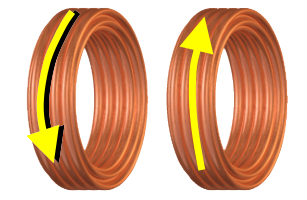
\includegraphics[width = 0.2\textwidth, height= 0.15\textwidth]{antiHelmholtz} 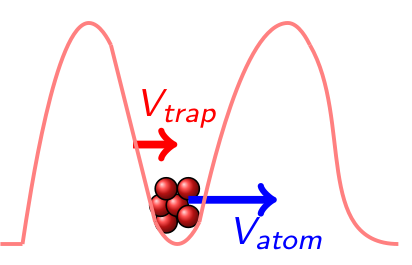
\includegraphics[width = 0.2\textwidth, height= 0.22\textwidth]{trap} 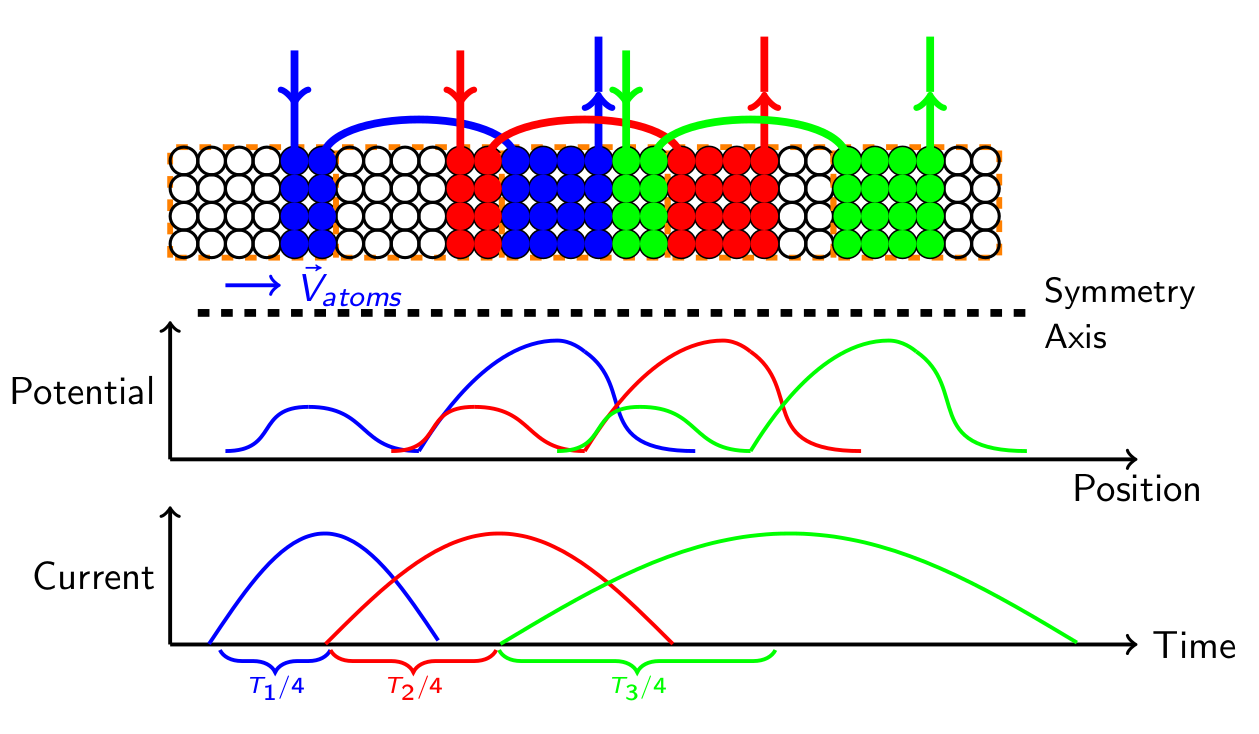
\includegraphics[width = 0.5\textwidth, height=0.22\textwidth]{switching} \caption{(A) Anti-Helmholtz coil. (B) Atoms in the magnetic trap. (C) Schematic for generating co-moving magnetic trap} \label{fig1} \end{figure}


\end{document}

